%!TEX root = draft.tex

\begin{figure*}[t]
	\vspace{-25pt}
	\centering
	\makebox[\textwidth][c]{\includegraphics[width=\textwidth]{final_final_exp}}
	\vspace{-16pt}
	\caption{
		Modeling network structure. We assess the extent to which network models
		fit key structural properties of six real-world networks. Tables 5A, 5B and 5C
		measure the accuracy of eight models in fitting the in-degree distribution,
		local clustering distribution, in-degree \& clustering relationship
		respectively and global attribute assortativity.
		%  Models with green \checkmark fit the assortativity
		% coefficient of attributed networks ---\texttt{ACL}, \texttt{APS} and
		% \texttt{Patents}--- up to 2 decimal places.
		% % We group models based on their
		% underlying edge formation mechanisms: preferential attachment, triangle closing
		% or random walks.
		Existing models tend to underperform because they either disregard
		the effect of factors such as triadic closure and/or homophily
		or are unable to generate networks with varying structural properties.
		Our model, \texttt{ARW}, jointly preserves all three properties accurately and often
		performs considerably better than existing models:
		the cells are shaded gray or dark gray if the proposed model \texttt{ARW} performs
		better at significance level $\alpha=0.01$ ( \lightgraybg{ }) or $\alpha=0.001$ ( \darkgraybg{ })
		respectively.
		% properties based on clustering. Models equipped with triangle closing
		% mechanisms ---\texttt{HK}, \texttt{SAN}---are not flexible enough to
		% accurately fit the skewed local clustering distributions of real-world
		% networks. Existing random walk models \texttt{FF}, \texttt{SK} and
		% \texttt{HZ} perform poorly because they are not expressive enough to
		% generate networks with varying structural properties.
	}
	\vspace{-10pt}
	\label{fig:exp_table}
\end{figure*}

\section{Experiments}
\label{sec:Experiments}
In this section, we evaluate the effectiveness of \texttt{ARW} in preserving
structural properties of network datasets described in~\Cref{sec:Datasets}.
relative to eight state-of-the-art growth models.
In~\Cref{sub:Experimental Setup}, we begin by describing existing growth models and the evaluation metrics
used in the experiments. Then, we discuss our results.

\subsection{Setup}
\label{sub:Experimental Setup}

% We first briefly summarize the existing models used in the experiments.
In this subsection, we describe the evaluation metrics used to quantify the extent to
which the following growth models preserve global structural properties of real-world networks.

\textit{State-of-the-art Growth Models}. We compare \texttt{ARW} to eight state-of-the-art
growth models representative of the key edge formation
mechanisms: preferential attachment, fitness, triangle closing and random walks.
Two of the following eight models account for attribute homophily and preserve attribute mixing patterns,
as listed in~\Cref{table:models}.

\begin{enumerate}
	\item{\textbf{Dorogovtsev-Mendes-Samukhin model}} \cite{dorogovtsev2000structure}  (\texttt{DMS})
	is a preferential attachment model in which the probability of linking to a node is proportional
	to the sum of its in-degree and ``initial attractiveness.''

	\item{\textbf{Kim-Altmann model}} \cite{kim2017effect} (\texttt{KA}) is a fitness-based model that defines
	fitness as the product of degree and attribute similarity. It can generate \textit{attributed} networks with assortative mixing and
	heavy tailed degree distribution.

	\item{\textbf{Relay Linking model}} \cite{singh2017relay} (\texttt{RL}) propose a set of
	preferential attachment models that use relay linking to explain the change in node popularity over time.
	\footnote{We use the iterated preferential relay-cite (IPRC) variant, which best fits real-world network properties}

	\item{\textbf{Holme-Kim model}} \cite{holme2002growing} (\texttt{HK}) is a preferential attachment model
	which uses a triangle-closing mechanism to generate scale-free, clustered networks.

	\item{\textbf{Social Attribute Network model}} \cite{gong2012evolution} (\texttt{SAN}) generates
	scale-free, attributed networks with high clustering using attribute-augmented
	preferential attachment and triangle closing mechanisms.

	% We modify the model
	% to create directed edges and thereby generate directed networks.

	\item{\textbf{Herera-Zufiria model}} \cite{saramaki2004scale} (\texttt{SK})  is a random walk model
	that tunes the length of random walks to generate clustered networks with power law degree distributions.

	\item{\textbf{Saramaki-Kaski}} \cite{herrera2011generating} (\texttt{HZ}) is a random walk model
	that generates scale-free networks with tunable average local clustering.

	\item{\textbf{Forest Fire model}} \cite{leskovec2005graphs} (\texttt{FF}) is a recursive random walk model
	that preserves decreasing diameter over time, heavy-tailed degree distribution
	and high clustering.
\end{enumerate}

\begin{table}[t]
 \center
 {
  \begin{tabular}[c]{llcc} \toprule
  Model &  Abbreviation & Type & Attributed \\ \midrule
  Dorogovtsev et al.~\cite{dorogovtsev2000structure} & \texttt{DMS} & \texttt{PA} & No  \\
  Relay Linking~\cite{singh2017relay} 						  & \texttt{RL} & \texttt{PA} & No  \\
  Kim-Altmann~\cite{kim2017effect} 							  & \texttt{KA} & \texttt{PA} & Yes  \\ \midrule
  Social Attribute Network~\cite{gong2012evolution} 	  & \texttt{SAN} & \texttt{PA+TC} & Yes  \\
  Holme-Kim~\cite{holme2002growing} 						  & \texttt{HK} & \texttt{PA+TC} & No  \\ \midrule
  Herera-Zufiria~\cite{herrera2011generating} 				  & \texttt{HZ} & \texttt{RW} & No  \\
  Saramaki-Kaski~\cite{saramaki2004scale} 					  & \texttt{SK} & \texttt{RW} & No  \\
  Forest Fire~\cite{leskovec2005graphs} 					  & \texttt{FF} & \texttt{RW} & No  \\
   \bottomrule
  \end{tabular}
  \vspace{1mm}
  \caption{
  	  We evaluate the performance of our model \texttt{ARW} relative to 3 preferential attachment
	  (\texttt{PA}) models, 2 pref. attachment \& triangle closing (\texttt{PA+TC}) models and 3 random walk (\texttt{RW}) models.
  }
  \label{table:models}
 }
 \vspace{-10pt}
\end{table}
\textit{Ensuring Fair Comparison}. To ensure fair comparison, we modify models outlined in~\Cref{table:models}.
First, for models that do not have an explicitly defined initial graph ---\texttt{DMS}, \texttt{SAN}, \texttt{KA}--- we use the
initialization method used for \texttt{ARW}, described in~\Cref{sub:Model Fitting}. Second, we extend
models that use constant node outdegree $m$, by increasing outdegree over time $m(t)$,
using the method described in~\Cref{sub:Model Fitting}. Third, we adjust models that generate undirected networks to
create directed edges and generate directed networks.

\textit{Evaluation}.
A network model fit should
preserve the global network structure of the observed network $G$.
We evaluate
the network model fit by comparing four key global network properties of ${G}$ and $\hat{G}$:
degree distribution, local clustering distribution, degree-clustering relationship
and attribute assortativity.
We use the Kolmogorov-Smirnov (\texttt{KS}) statistic to compare the univariate degree
\& local clustering distributions.
% We use absolute difference to compare the
% attribute assortativity coefficients of networks $G$ and $\hat{G}$.
We compare the bivariate degree-clustering relationship in $G$ and $\hat{G}$ using
Weighted Relative Error (\texttt{WRE}). The evaluation metric \texttt{WRE} aggregates the relative error
between the average local clustering $c(k)$ and $\hat{c}(k)$ of nodes  with in-degree $k$
in $G$ and $\hat{G}$ respectively; The weight of each relative error term equals the fraction
of nodes with in-degree $k$ in $G$.

Jointly preserving multiple structural properties is a multi-objective optimization
problem; Model parameters that accurately preserve the degree distribution
(i.e. low \texttt{KS} statistic) may not preserve the clustering distribution.
Therefore, for each model, we use grid search to select the model parameters
that minimizes the $\ell^2$-norm of the evaluation metrics. The sensitivity of the
Forest Fire model requires a manually guided grid search method. Since the metrics have
different scales, we normalize the metrics before computing the $\ell^2$-norm
to prevent any bias towards a particular metric.
Next, we evaluate the performance of \texttt{ARW} in preserving multiple structural
properties of six network datasets, relative to state-of-the-art existing models outlined
in this subsection.

\subsection{Results}
\label{sub:Experimental Results}

Now, we evaluate the performance of \texttt{ARW} relative to eight well-known
existing models on the datasets introduced in~\Cref{sec:Datasets}.

To evaluate the performance of network models, we first fit every model
to each network dataset $G$. Thereafter, we compare the structural properties of
network dataset $G$ and network $\hat{G}$ generated by the fitted model using
evaluation metrics introduced in~\Cref{sub:Experimental Setup}. We average out
fluctuations in $\hat{G}$ over 100 runs; data from these runs also help us conduct statistical tests.

\Cref{fig:exp_table} lists the evaluation metrics for every pair of model
and dataset. The metrics measure the accuracy with which these models
preserve key global network properties: degree distribution, local clustering distribution,
and indegree-clustering relationship. We do not compare the extent to which these models preserve attribute assortativity because the attribute related model parameters can be independently tuned to obtain arbitrary assortativity precision. Instead, we indicate models that preserve assortativity up to two decimal
places---\texttt{KA}, \texttt{SAN} and \texttt{ARW}---by green ticks (\checkmark) in~\Cref{fig:exp_table}.

We use permutation tests \cite{good2013permutation} to evaluate the relative
performance of \texttt{ARW}. If
\texttt{ARW} performs better than a model on a dataset with significance level
$\alpha=0.01$ or $\alpha=0.001$, the corresponding cells in~\Cref{fig:exp_table}
are shaded gray ( \lightgraybg{ }) or dark gray (~\darkgraybg{ }) respectively.

% The performance of a model depends on the effectiveness of its underlying
% edge formation mechanisms. To study the strengths and weaknesses of these mechanisms,
% we group models (i.e. color-coded rows in table \ref{fig:exp_table}) based on their
% underlying edge formation mechanism: preferential attachment (blue), preferential attachment with
% triangle closing (orange) and random walk (green) mechanisms.

% A common characteristic of
~\Cref{fig:exp_table} shows that existing models fail to accurately preserve
{multiple} structural properties. This is because existing models either
disregard important mechanisms such as triadic closure and homophily or are not
flexible enough to generate networks with varying structural properties.

% For instance, the preferential attachment model \texttt{DMS}
% can accurately fit the heavy-tailed degree distributions but does not
% account for local clustering.
% On the other hand, the attributed network model \texttt{SAN} tries to preserve
% all four properties but cannot do so accurately.

\textbf{Preferential attachment models}: \texttt{DMS}, \texttt{RL}
and \texttt{KA} preserve in-degree distributions but disregard
clustering. \texttt{DMS} outperforms other models in accurately modeling
degree distribution (\Cref{fig:exp_table}A) because its ``initial attractiveness''
parameter can be tuned to adjust preference towards low degree nodes. Unlike \texttt{KA}, however,
\texttt{DMS} cannot preserve global assortativity.
\texttt{KA} outperforms \texttt{DMS} in preserving global assortativity because \texttt{KA}
uses an attribute similarity parameter to model attribute mixing patterns.
By assuming that successive edge formations are independent, both models disregard
triadic closure and local clustering. (\Cref{fig:exp_table}B \&~\Cref{fig:exp_table}C).

\textbf{Triangle Closing Models}: \texttt{HK} and \texttt{SAN} are preferential attachment models
that use triangle closing mechanisms to generate scale-free networks with high average
local clustering.
Note that \texttt{HK} and \texttt{KA} fit degree distributions with the same \texttt{KS} statistic
(\Cref{fig:exp_table}A) because they lack parameters that can generate varying degree distributions.
While triangle closing leads to considerable improvement over \texttt{DMS}
and \texttt{KA} in modeling local clustering, \texttt{HK} and \texttt{SAN} are not flexible enough
to preserve local clustering in {all} datasets (see~\Cref{fig:exp_table}B \&~\Cref{fig:exp_table}C).
%  Nevertheless,
% barring one or two datasets in tables \ref{fig:exp_table}B and \ref{fig:exp_table}C,
% these models cannot accurately preserve the local clustering distribution and in-degree-clustering
% relationship observed in real networks.

\textbf{Existing random walk models}: \texttt{FF}, \texttt{SK}, and \texttt{HZ}
do not accurately preserve structural properties of real-world network datasets,
disregard attribute homophily and do not account for attribute mixing patterns.
The recursive approach in \texttt{FF} considerably overestimates local clustering
because nodes perform a probabilistic breadth-first search and link to \textit{all} visited/burned
nodes.
In \texttt{SK} and \texttt{HZ}, nodes perform a single random walk and link to
each visited node with some probability $\mu$, which indirectly
controls the effect on triadic closure. This leads to some improvement over \texttt{FF} in preserving local
clustering distribution (\Cref{fig:exp_table}B) and in-degree-clustering relationship (\Cref{fig:exp_table}).
% However, the improvements are not substantial when compared to the performance
% of our model \texttt{ARW}.

\textbf{Attributed Random Walk model}: The results in~\Cref{fig:exp_table} clearly indicate the effectiveness
of the proposed model \texttt{ARW} in {jointly} preserving multiple
global network properties. \texttt{ARW} can generate networks with varying
in-degree distribution by adjusting nodes' preference towards high degree nodes
using outlink parameter $p_o$. As a result, \texttt{ARW} accurately preserves
degree distribution (\Cref{fig:exp_table}A), often significantly better
than all models except \texttt{DMS}. Similarly, \texttt{ARW} matches the local clustering
distribution  (\Cref{fig:exp_table}B) and in-degree \& clustering relationship
(\Cref{fig:exp_table}C) with high accuracy because the jump parameter $p_j$ and
link parameter $p_l$ in \texttt{ARW} control the effect of triadic closure.
The attribute parameter $p_a$ can be tuned to match the attribute assortativity
coefficient of attributed network datasets up to arbitrary precision.
Barring one to two datasets, \texttt{ARW} preserves all three properties significantly
better ($\alpha < 0.001$) than existing random walk models.
From~\Cref{fig:barplot}, it is straightforward to show that
\texttt{ARW} improves upon the average $\ell^2$-norm of the second best performing model
\texttt{SAN} by a margin of 2.5x.


\begin{figure}
	\centering
	\vspace{-6pt}
	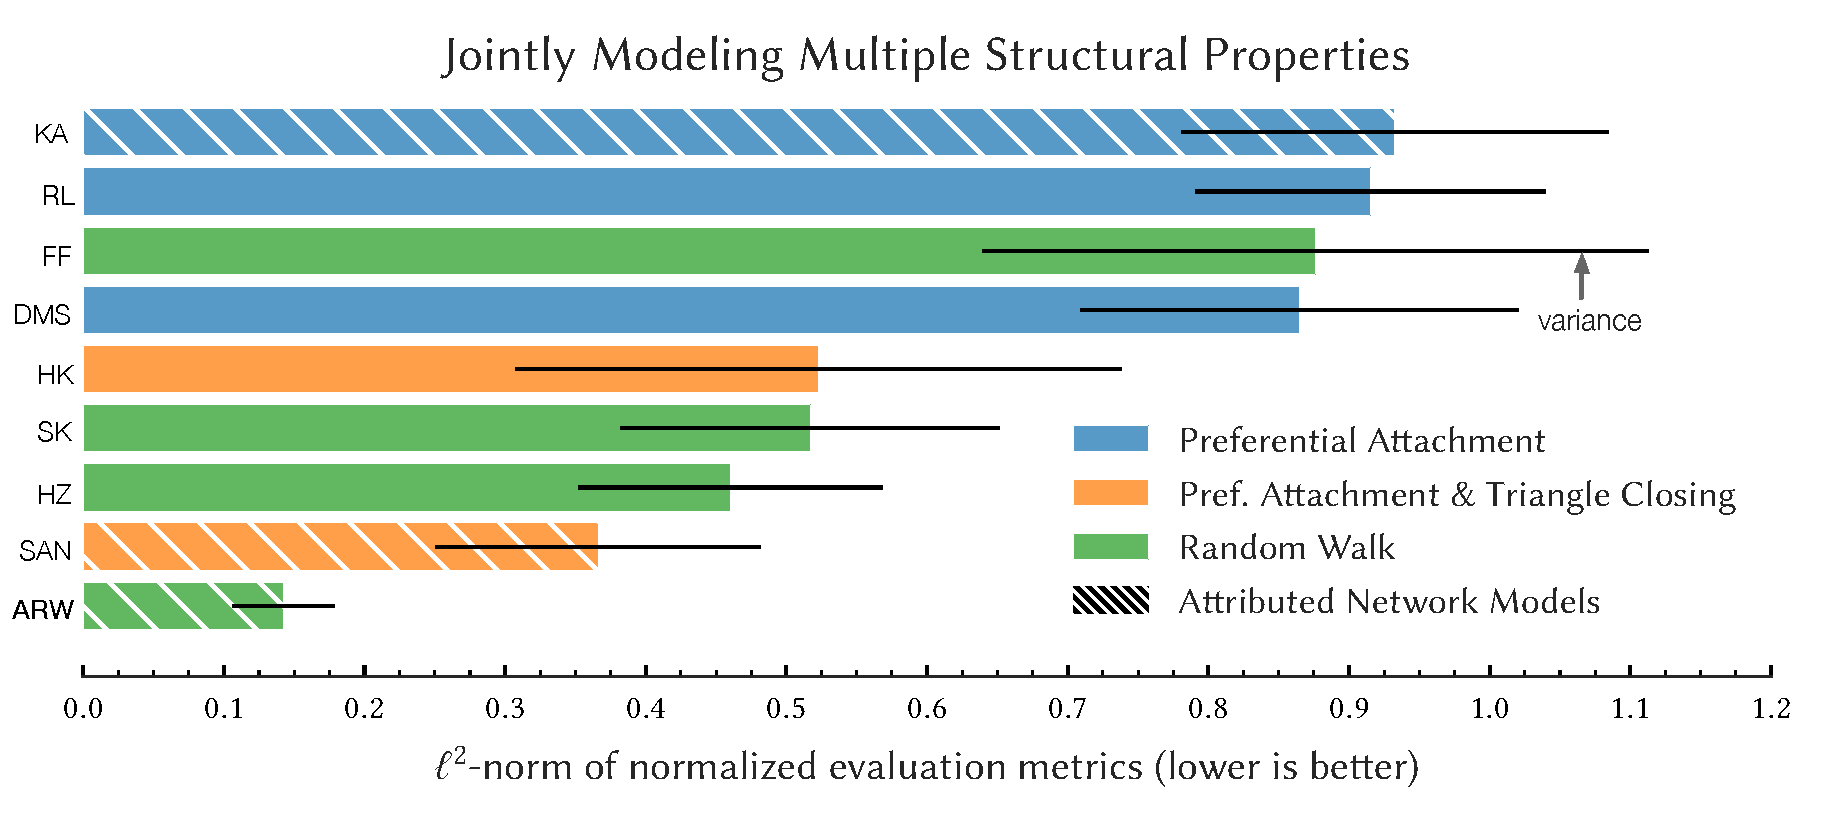
\includegraphics[width=\linewidth]{barplots_final4f}
	\caption{Jointly modeling multiple network properties: \texttt{ARW} outperforms
		existing network models in jointly preserving key structural properties---in-degree
		distribution, local clustering distribution and degree-clustering relationship---
		by a margin of 2.5x-10x.
	}
	\vspace{-8pt}
	\label{fig:barplot}
	% Existing network models perform poorly
	% because they make strong modeling assumptions that disregard individual resource constraints
	% and do not consider multiple factors that simultaneously influence edge formation.
\end{figure}

To summarize, \texttt{ARW} unifies multiple sociological phenomena
into a single mechanism. As a result, it can jointly preserve key structural
properties of real-world networks.


\Cref{fig:barplot} illustrates the performance of network models in jointly
modeling degree distribution, local clustering distribution and in-degree-clustering
relationship. Preferential attachment models \texttt{KA}, \texttt{DMS} and
\texttt{RL} perform poorly because they do not preserve clustering. \texttt{HK}
and \texttt{SAN} perform better than \texttt{KA}, \texttt{DMS} and
\texttt{RL} because of edge formation mechanisms that close triangles
to preserve clustering and its relationship with degree to some extent. The proposed
model \texttt{ARW} outperforms existing random walk models \texttt{HZ}, \texttt{SK}
and \texttt{FF} by a considerable margin.
\texttt{ARW} significantly improves upon the average $\ell^2$-norm of the second best performing model,
\texttt{SAN} by a margin of 2.5x.


% As shown in \cref{fig:barplot},
% \texttt{ARW} improves upon the average $\ell^2$-norm of the second best performing model,
% \texttt{SAN} by a margin of 2.5x.


% In \Cref{fig:barplot}, we show that \texttt{ARW} performs considerably better than
% six state-of-the-art, representative network models in jointly modeling
% degree distribution, local clustering distribution and in-degree-clustering
% relationship.
% Preferential models \texttt{KA} and \texttt{DMS} perform poorly because
% they disregard clustering whereas the recursive approach in \texttt{FF} overestimates
% local clustering.
% Next, we discuss limitations
% of the global assortativity coefficient and analyze local mixing patterns of
% attributed networks.

% \clearpage
% \section{Modeling Local Mixing Patterns}
% \label{subsec:LocalMixing}
%
% The global assortativity coefficient quantifies
% % the level of homophily or heterophily in an attributed network. It sheds light
% % on
% the average propensity of links to occur between similar nodes
% %  by capturing
% % the attribute mixing pattern across the entire network.
% However, global assortativity is not a representative summary statistic of heterogeneous mixing patterns observed in large-scale networks~\cite{peel2018multiscale}. Furthermore, It does not quantify anomalous mixing patterns and fails to measure how mixing varies across a network.
%
% We use local assortativity~\cite{peel2018multiscale} to measure varying
% mixing patterns in an attributed network $G=(V,E,B)$ with attribute values $B=\{b_1...b_h\}$.
% Unlike global assortativity that counts all edges between similar nodes, local assortativity of node $i$, $r_l(i)$, captures mixing pattern in the local neighborhood of node $i$ by using a locality biased weight distribution $w_i$. The distribution $w_i$ reweighs edges between similar nodes based on how local they are to node $i$. As~\citet{peel2018multiscale} indicate, there are multiple ways to define $w_i$, and we define $w_j = \sfrac{1}{d_i}, j \in N(i)$, as this allows for a highly efficient local assortativity calculation.
%
% % The distribution $w_i$ reweighs edges between similar nodes
% % based on how local they are to node $i$. Peel et al. \cite{peel2018multiscale} prescribe a
% % personalized pagerank weight distribution, which is prohibitively expensive to compute for
% % all nodes in large graphs; Large network datasets necessitate efficient weighting schemes.
% % Therefore, we define $w_i$ as a uniform distribution
% % over $N(i)$, the set of nodes that are at most 1 hop away from node $i$.
%
% % reintroduce only if there is room.
% % More formally, the local assortativity coefficient $r_l(i)$ of node $i$, with outdegree $m(i)$ and
% % attribute value $b(i)$ is defined as follows:
% % \vspace{-1mm}
% % \begin{align*}
% % 	\scriptsize r_l(i) = \frac{\overbrace{\frac{1}{|N(i)|}\sum\limits_{j \in N(i)}^{m(j) > 0} \sum_{k \in V} \frac{\mathcal{I}\{(j,k) \in E \wedge b(j)=b(k)\}}{m(i)} }^{\texttt{obs}}-\overbrace{\sum_{b \in B} e_{b}\cdot e_{b}}^{\texttt{rnd}}}{\underbrace{1}_{\max(\texttt{obs})}-\underbrace{\sum_{b \in B} e_{b} \cdot e_{b}}_\texttt{rnd}}
% % \end{align*}
% % Intuitively, $r_l(i)$ compares the observed fraction of edges between similar nodes
% % in the local neighborhood of node $i$ (\texttt{obs}) to the expected fraction
% % if the edges are randomly rewired (\texttt{rnd}).
%
% The local assortativity distributions
% of \texttt{ACL}, \texttt{APS} and \texttt{Patents} reveal anomalous, skewed
% and heterophilic local mixing patterns that are not easily inferred via the global assortativity,
% as shown in \cref{fig:local_atty}.
% \begin{figure}
% 	\centering
% 	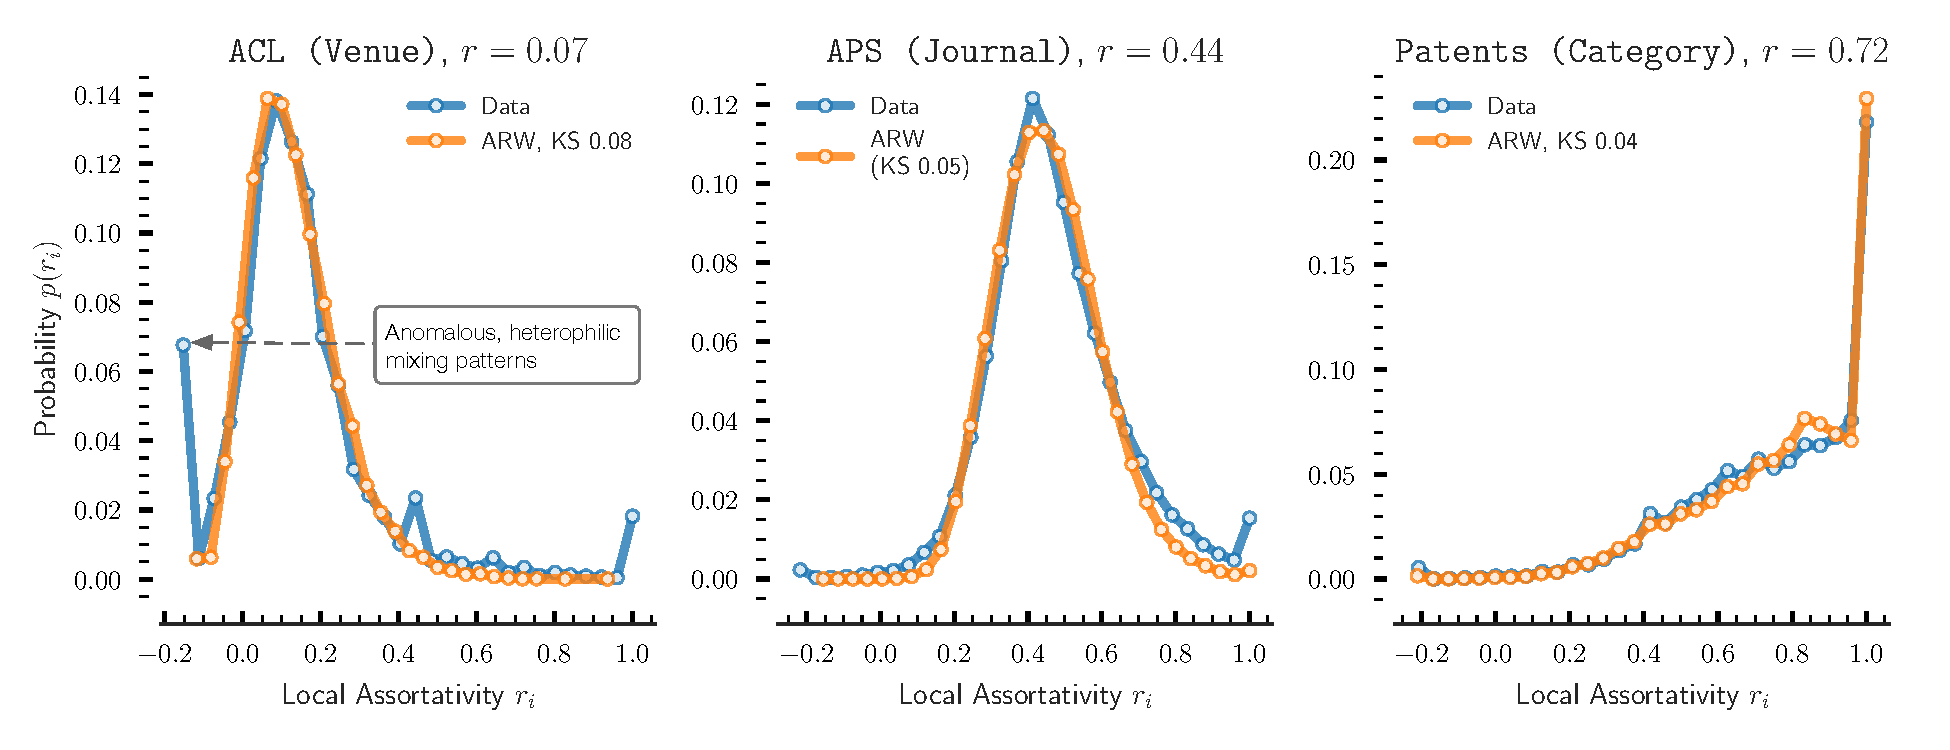
\includegraphics[width=\linewidth]{local_atty_dist}
% 	\caption{Local attribute mixing patterns of homophilic networks \texttt{ACL}, \texttt{APS}
% 		and \texttt{Patents} reveal anomalous, skewed and even heterophilic local mixing patterns.
% 		\texttt{ARW} preserves the observed local assortativity distributions with high accuracy,
% 	but does not account for nodes with extreme heterophilic or homophilic preferences.}
% 	\label{fig:local_atty}
% \end{figure}
% \texttt{ARW} can preserve
% diverse local assortativity distributions with high accuracy even though nodes
% share the same attribute preference parameter $p_a$. This is because  \texttt{ARW}
% incorporates multiple sources of stochasticity through its edge formation
% mechanism. As a result, incoming nodes with fixed homophilic preferences can end
% up having variable local assortativity by (a) selecting a seed node in a region
% with too few (or too many) similar nodes or (b) exhausting all its links before
% visiting similar (or dissimilar) nodes.
% \texttt{ARW} is not expressive enough to accurately model anomalous
% mixing patterns. Mechanisms such as sampling $p_a$ from a mixture of
% Bernoulli distributions are necessary to account for anomalous mixing patterns.

% The local assortativity coefficient $r_l(i)$ of node $i$,
% with outdegree $k(i)$ and attribute value $b(i)$, uses a distribution $w_i$ to
% reweigh edges based on how local they are to node $i$:
% \begin{equation*}
%     r_l(i) = \frac{\sum\limits_{b \in B} e_{bb}(i) - \sum\limits_{b \in B} e_{b.}e_{.b}}{1 - \sum\limits_{b \in B} e_{b.}e_{.b}}
% \end{equation*}


%
% Unlike global assortativity, local assortativity coefficient of node $i$,
% $r_l(i)$, compares the mixing patterns in node $i$'s locality to the expected
% mixing pattern if the edges were randomly rewired.
% Given a directed network $G=(V,E)$ with adjacency matrix $A$ and attribute
% values $B=\{b_1...b_m\}$, the local assortativity coefficient $r_l$ of node $i$
% with outdegree $k_i$ is defined as follows:
%

% can generate network
% with tunable local clustering distribution and in-degree-clustering relationship
% controls the effect of triadic closure using the jump parameter $p_j$ and link parameter
% $\alpha$. $p_j$ effectively incorporates structural constraints that limit the extent to
% which nodes explore the network whereas $\alpha$ indirectly controls the effect of
% triadic closure on edge formation.

% \subsection{Parameter space of \textsc{RW} model}
%
% Through a series of extensive experiments, we observe that our model \textsc{RW} is able
% to model multiple structural characteristics of real-world networks. However, the fitted
% parameters are different for each dataset, suggesting possibly different
% local growth mechanisms in each network.~\Cref{table:rw_parameters}
% describes the best fitted parameters for five citation networks used in
% our experiments.
%
%
% \begin{table}[!h]
% \center
% \caption{ Best fittedparameters obtained after grid search for random walk model. }
% \label{table:rw_parameters}
% \resizebox{\columnwidth}{!}{%
% \begin{tabular}{@{}cccccc@{}}
%  & \multicolumn{1}{c}{\textit{USSC}} & \multicolumn{1}{c}{\textit{HEP-PH}}& \multicolumn{1}{c}{\textit{APS}}& \multicolumn{1}{c}{\textit{Patents}} & \multicolumn{1}{c}{\textit{Semantic}} \\ \toprule
%  $p_l$ & 0.80 & 0.80 & 0.15 & 0.25 & 0.40 \\
%  $p_j$ & 0.30 & 0.65 & 0.65 & 0.05 & 0.15 \\
%  $p_o$ & 0.95 & 0.95 & 0.80 & 1.00 & 0.95 \\
%  $p_r$ & 0.50 & 0.80 & 0.85 & 0.45 & 0.60 \\ \midrule
% \end{tabular}
% }
% \end{table}

% To summarize, the experiment results on five citation networks against
% show that our resource-constrained model (\textsc{rw}) outperform four existing
% growth models in accurately preserving degree, clustering and its relationship.

% Weighted relative error (\texttt{WRE})
% is used to measure the similarity between the in-degree \& local clustering relationship in $G$ and $\hat{G}$:
% $$ \texttt{WRE}: \sum_{\text{Indeg.} k} P_{\textsc{g}}(k) \frac{c(k)-\hat{c}(k)}{c(k)} $$
% \texttt{WRE} is the weighted sum of the relative error between $c(k)$ and $\hat{c}(k)$,
% the average local clustering of nodes with degree $k$ in $G$ and $\hat{G}$ respectively;
% which aggregates the relative error between $c(k)$ and $\hat{c}(k)$,
% the average local clustering of nodes with degree $k$ in networks $G$
% and $\hat{G}$ respectively; The weight of each relative error term equals the probability
% mass $p_G(k)$ of in-degree $k$ in the observed network $G$.

%
% \begin{figure*}
%  \centering
%  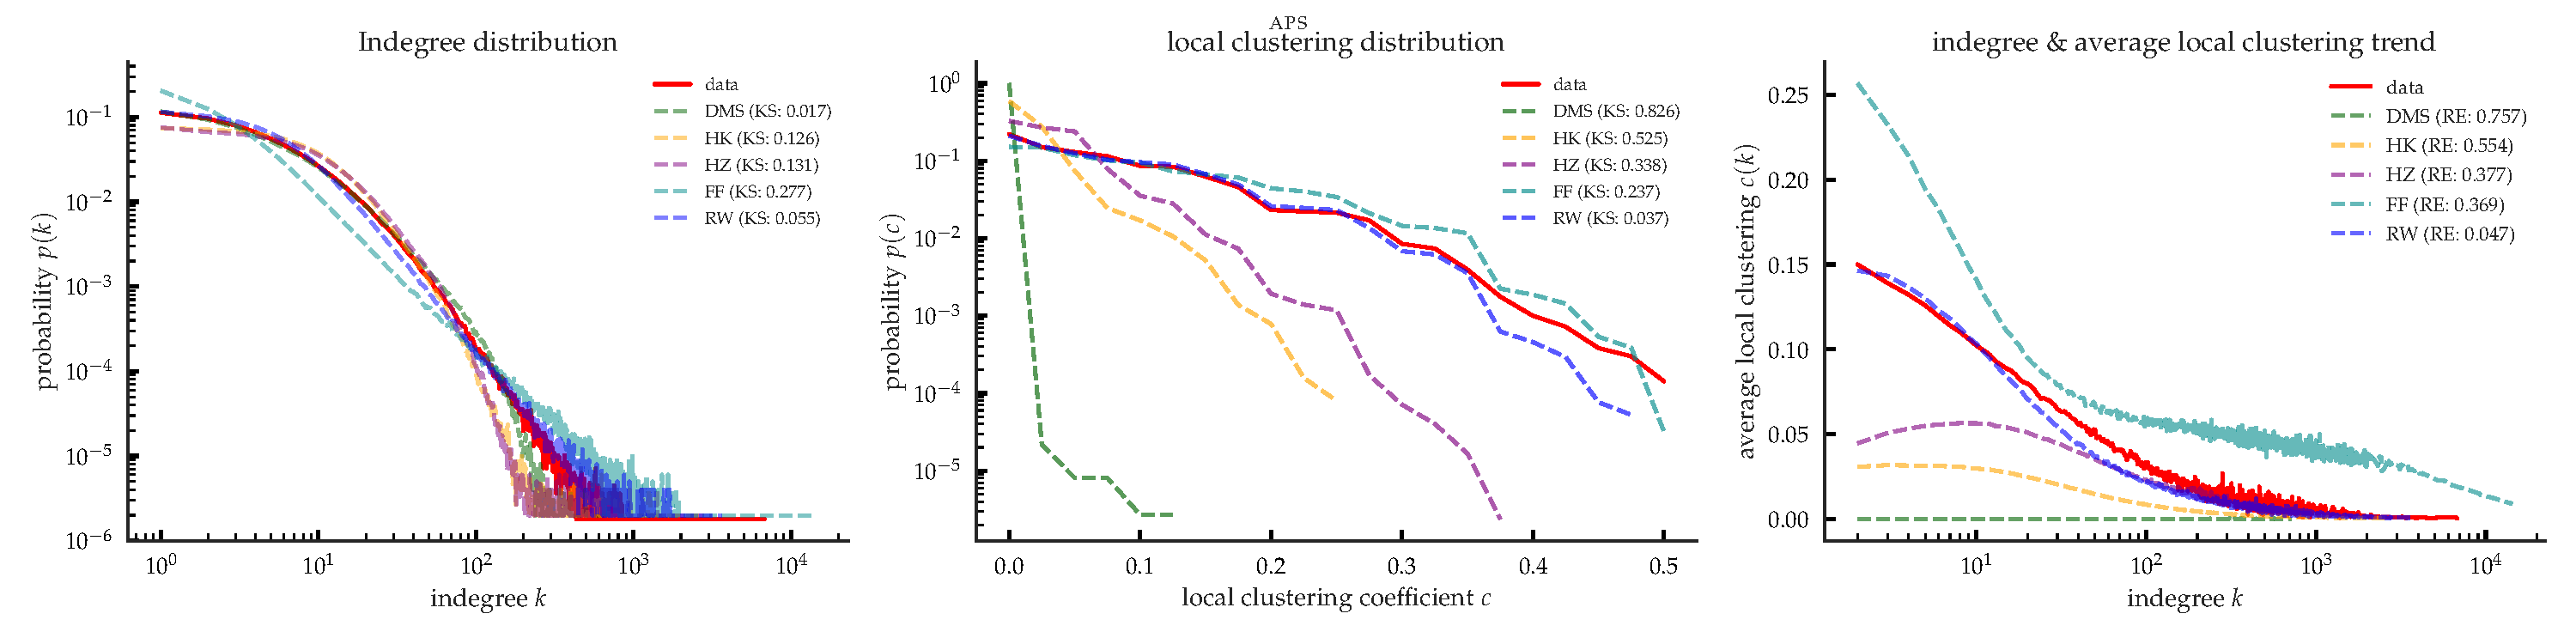
\includegraphics[width=\textwidth]{exp_aps}
%  \vspace{-12pt}
%
% \caption{Accuracy of growth models at preserving structural properties of \textsc{APS} network.
%  Our model \textsc{rw} outperforms the other in \textit{jointly} preserving heavy-tailed in-degree
%  distribution, skewed local clustering distribution and the in-degree \& average local clustering trend.}
%
% \label{fig:analysis}
% \end{figure*}

